% !TEX root = ../Dissertation.tex
\section{Basics of Reinforcement Learning}
\label{sec:rl}

Given the inherent limitations of both exact algorithms and traditional heuristics for solving large-scale combinatorial optimization problems, this research turns to Reinforcement Learning (RL) as a promising alternative paradigm.
The idea of using neural networks for optimization problems dates back to early work on Hopfield networks \cite{hopfieldNeuralComputationDecisions1985}. However, it is the recent breakthroughs in deep reinforcement learning, such as the development of Deep Q-Networks that achieved human-level control on Atari games \cite{mnihHumanlevelControlDeep2015}, that have truly enabled the creation of powerful, end-to-end solvers for COPs \cite{khalilLearningCombinatorialOptimization2017}.

\subsection{Why Reinforcement Learning?}

The motivation for employing RL is best understood by comparing it to other dominant approaches for solving complex problems: supervised learning, commercial solvers, and metaheuristics.
\begin{itemize}
    \item \textbf{In Comparison to Supervised Learning (SL):} The primary advantage of RL is its independence from large datasets of high-quality, labeled solutions.
For a problem like the 0/1 Knapsack, generating such labels would require running a commercial exact solver (e.g., Gurobi).
This presents a paradox: if a commercial solver can efficiently find the optimal solution to generate a label, the problem for that specific instance is already solved, rendering the training of an SL model for that purpose somewhat redundant.
RL circumvents this by learning directly from interaction and a scalar reward signal.
However, it is worth noting that SL can be synergistically combined with RL, for instance, by using imitation learning to pre-train an agent from expert (solver-generated) demonstrations to accelerate the learning process.
\item \textbf{In Comparison to Commercial Solvers:} While solvers like Gurobi or CPLEX are powerful tools that guarantee optimality, their runtime often scales exponentially with problem size for NP-hard problems.
For very large or complex instances, finding the optimal solution can become computationally intractable.
Furthermore, they typically operate as deterministic "black boxes," offering less flexibility in stochastic or dynamic environments.
In contrast, a trained RL agent learns a \textit{policy}---a mapping from states to actions---that can generate high-quality solutions very quickly (often in constant or near-constant time) once trained, making it highly suitable for applications requiring rapid decision-making.
\item \textbf{In Comparison to Metaheuristics:} Algorithms like Genetic Algorithms (GA) or Simulated Annealing (SA) provide another alternative.
However, their performance is highly sensitive to a set of hyperparameters that require extensive, problem-specific tuning.
Crucially, these parameters often need to be re-tuned when the scale or characteristics of the problem instances change.
Moreover, they can be prone to premature convergence to local optima.
An RL model, once successfully trained, encapsulates a generalized solving strategy.
It can be invoked directly to solve any problem instance within the distribution it was trained on, up to a specified maximum scale, without the need for re-tuning for each new instance.
\end{itemize}

\subsection{What is Reinforcement Learning?}

Reinforcement Learning is a paradigm of machine learning where an \textit{agent} learns to make a sequence of optimal decisions by interacting with an \textit{environment}.
The agent's goal is to learn a policy that maximizes a cumulative reward signal over time.
This interaction is typically modeled as a Markov Decision Process (MDP).
The core of RL is the agent-environment interaction loop, as depicted in Figure~\ref{fig:ae_loop}.
At each timestep \(t\), the agent observes the environment's state \(S_t\) and, based on its policy, selects an action \(A_t\).
The environment transitions to a new state \(S_{t+1}\) and provides the agent with a scalar reward \(R_{t+1}\) as feedback on its action.
This process repeats, allowing the agent to learn from the consequences of its actions.

\begin{figure}[htbp]
    \centering
    % Note: Ensure the path is correct relative to your main .tex file
    % If Dissertation.tex is in '.../dissertation/', this path should work.
    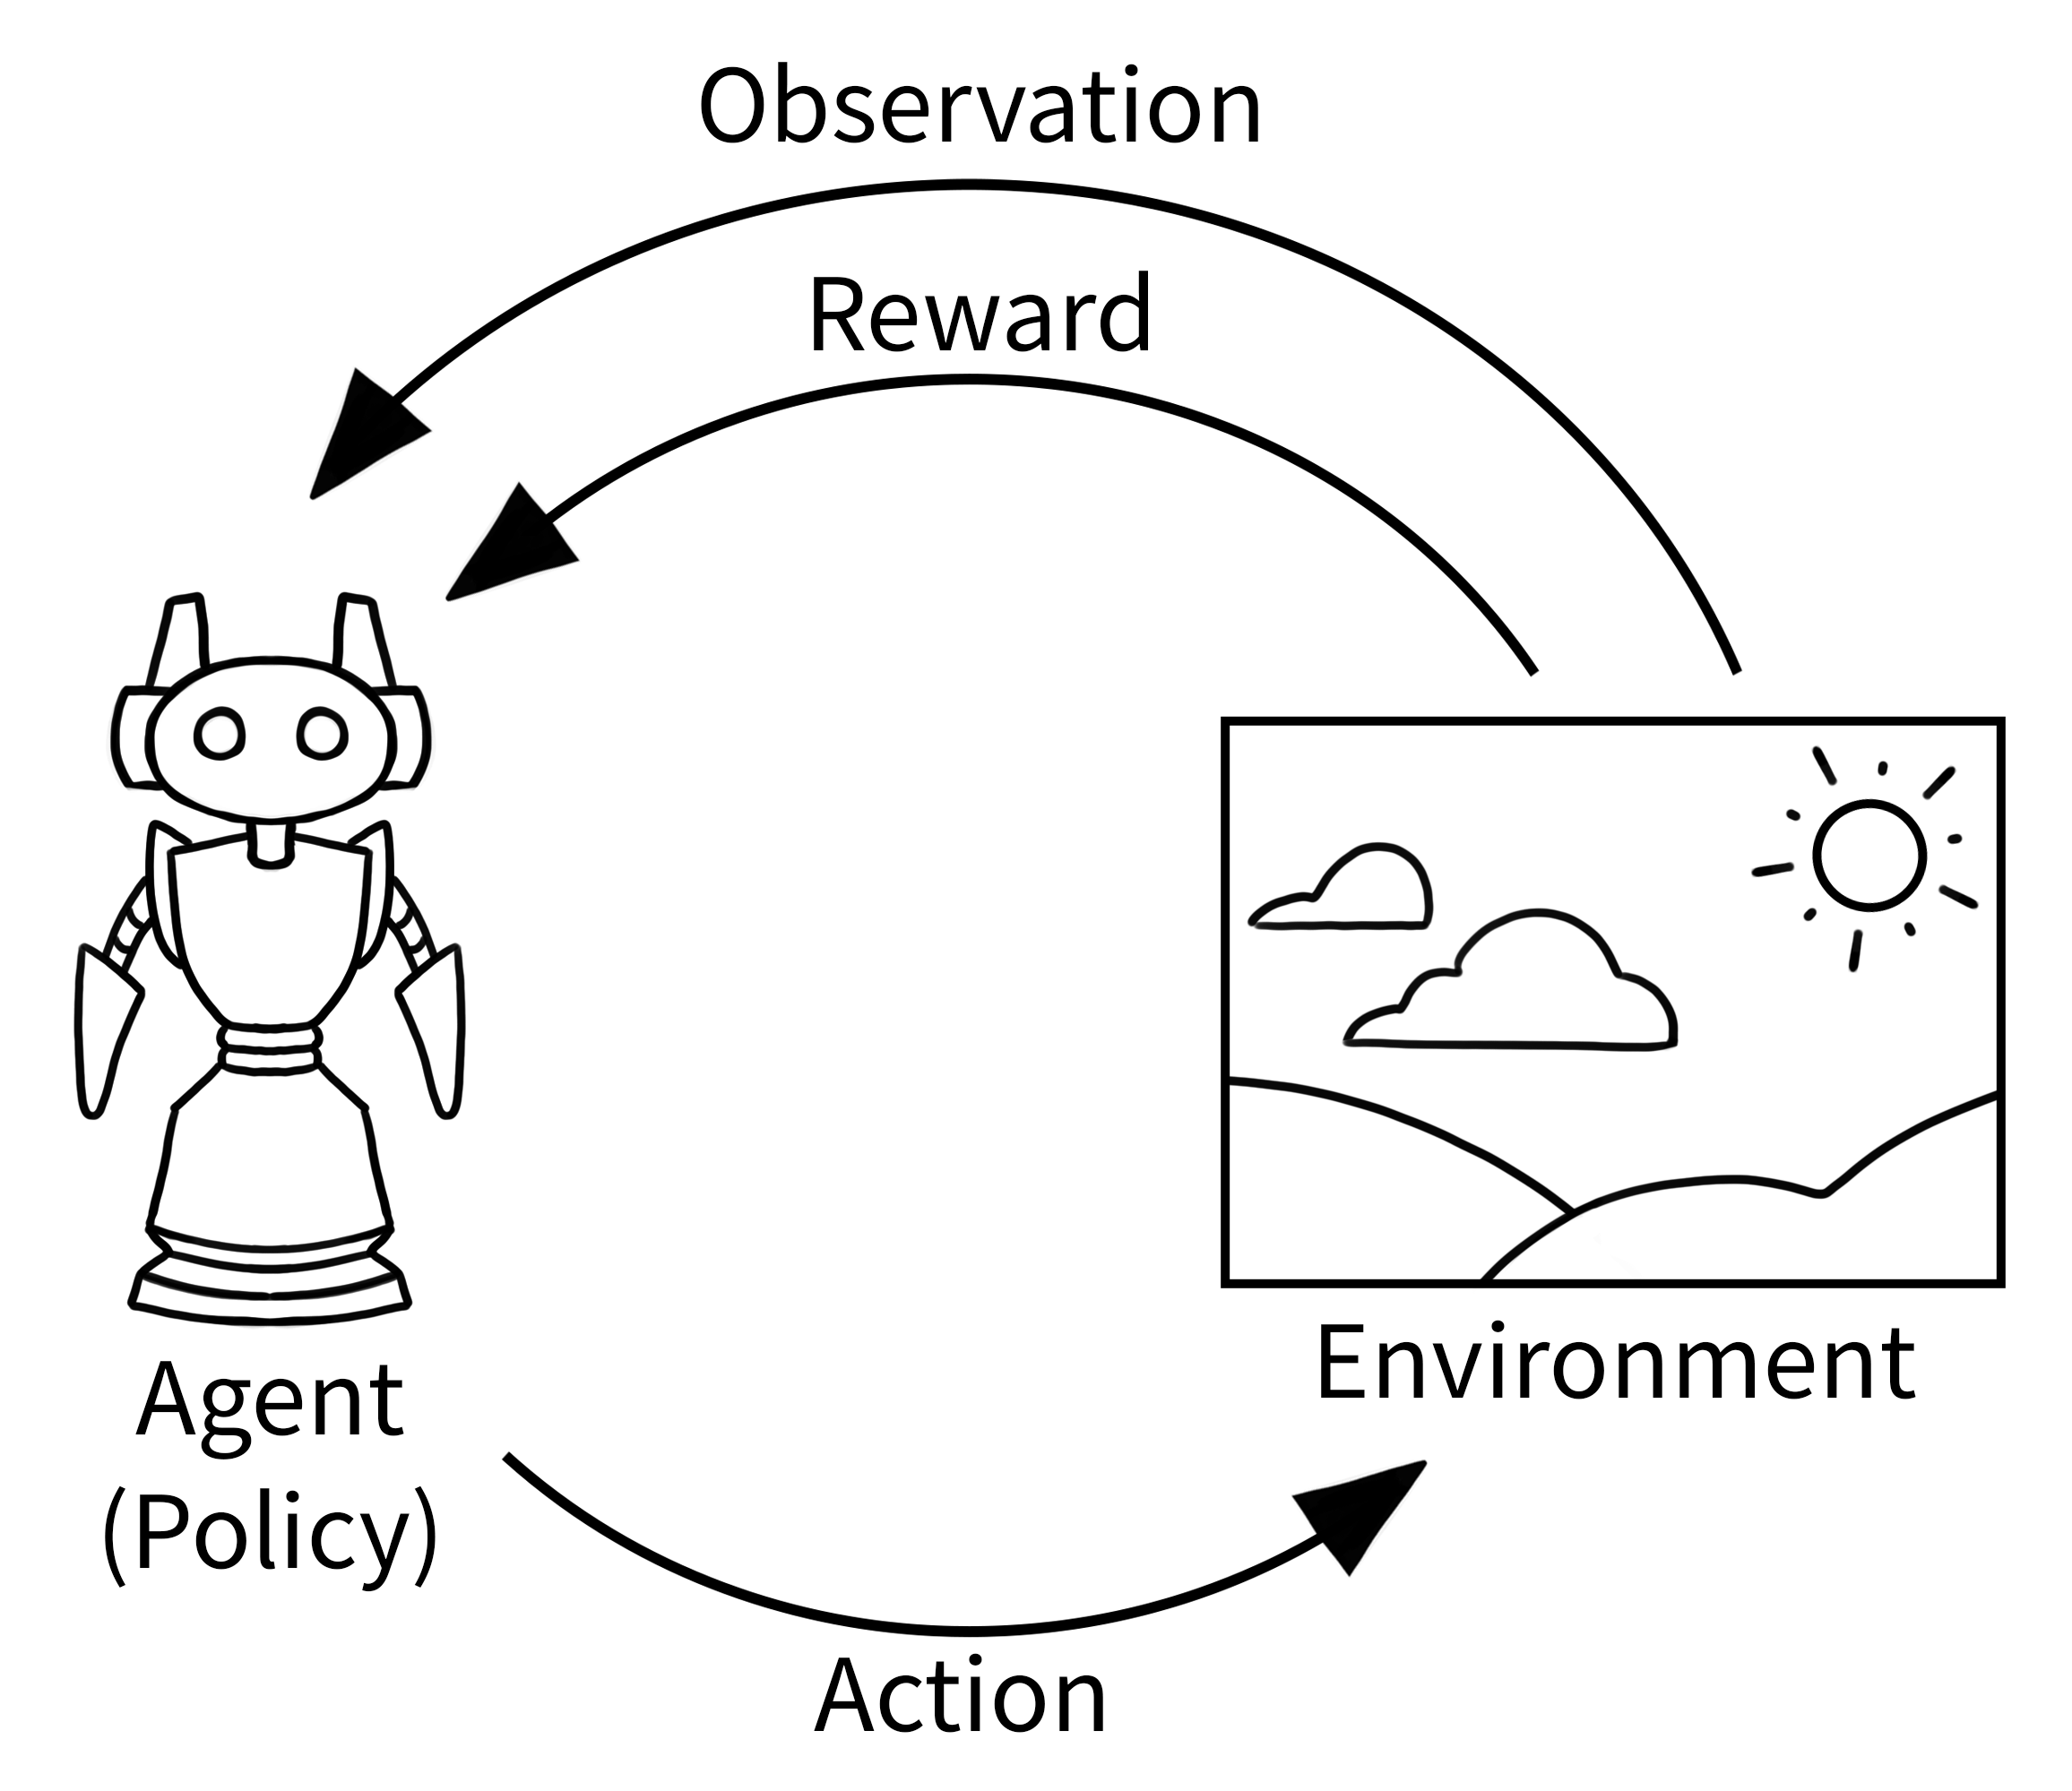
\includegraphics[width=0.8\textwidth]{figures/AE_loop.png}
    \caption{The standard agent-environment interaction loop in Reinforcement Learning. Source: Gymnasium Documentation.}
    \label{fig:ae_loop}
\end{figure}

A critical distinction from other machine learning paradigms is the nature of the training data.
The agent does not learn from a static dataset of raw problem data (e.g., item weights and values).
Instead, the learning process is driven by data generated dynamically through interaction.
This data takes the form of trajectories or experiences, which are sequences of tuples:
\[ (S_t, A_t, R_{t+1}, S_{t+1}) \]
By collecting these experiences, the agent refines its policy to favor actions that lead to higher long-term cumulative rewards.
For the Knapsack Problem, this means learning a sequence of item selections that ultimately yields the highest total value without violating the capacity constraint.